\documentclass[11pt,a4paper]{report}

% ─── Packages ───
\usepackage[utf8]{inputenc}
\usepackage[T1]{fontenc}
\usepackage[margin=1in, top=1.2in, bottom=1.2in]{geometry}
\usepackage{amsmath,amssymb,amsthm,mathtools}
\usepackage{xcolor}
\usepackage{titlesec}
\usepackage{titletoc}
\usepackage{fancyhdr}
\usepackage{enumitem}
\usepackage{tcolorbox}
\usepackage{booktabs}
\usepackage{graphicx}
\usepackage{hyperref}
\usepackage{cleveref}
\usepackage{tikz}
\usepackage{setspace}
\usepackage{parskip}
\usepackage{caption}
\usepackage{etoolbox}
\usepackage{array}
\usepackage{multirow}

\usetikzlibrary{arrows.meta, positioning, shapes.geometric, calc, decorations.pathmorphing, fit, backgrounds, chains}
\tcbuselibrary{skins,breakable,theorems}

% ─── Colors ───
\definecolor{darkindigo}{HTML}{1a237e}
\definecolor{accentcyan}{HTML}{00bcd4}
\definecolor{deepviolet}{HTML}{4a148c}
\definecolor{softgold}{HTML}{c8a951}
\definecolor{darkbg}{HTML}{0d0d1f}
\definecolor{sectionblue}{HTML}{1a3a5c}
\definecolor{subsecblue}{HTML}{2c5f8a}
\definecolor{defcolor}{HTML}{1565c0}
\definecolor{defbg}{HTML}{e3f2fd}
\definecolor{principlecolor}{HTML}{880e4f}
\definecolor{principlebg}{HTML}{fce4ec}
\definecolor{mechcolor}{HTML}{4a148c}
\definecolor{mechbg}{HTML}{f3e5f5}
\definecolor{mathbg}{HTML}{f8f5ee}
\definecolor{notepurple}{HTML}{7b1fa2}
\definecolor{notebg}{HTML}{f3e5f5}
\definecolor{lightgray}{HTML}{f0f0f0}
\definecolor{darkgray}{HTML}{333333}
\definecolor{predcolor}{HTML}{e65100}
\definecolor{predbg}{HTML}{fff3e0}
\definecolor{compcolor}{HTML}{00695c}
\definecolor{compbg}{HTML}{e0f2f1}
\definecolor{varcolor}{HTML}{bf360c}
\definecolor{varbg}{HTML}{fbe9e7}
\definecolor{objcolor}{HTML}{1b5e20}
\definecolor{objbg}{HTML}{e8f5e9}

% ─── Hyperref Setup ───
\hypersetup{
    colorlinks=true,
    linkcolor=darkindigo,
    citecolor=darkindigo,
    urlcolor=deepviolet,
    bookmarks=true,
    bookmarksnumbered=true,
    pdfauthor={Comprehensive Guide},
    pdftitle={Higher-Order Theories of Consciousness (HOT)},
    pdfsubject={Consciousness, Philosophy of Mind, Metacognition, Neuroscience},
}

% ─── Header/Footer ───
\pagestyle{fancy}
\fancyhf{}
\fancyhead[L]{\small\color{gray} Higher-Order Theories of Consciousness}
\fancyhead[R]{\small\color{gray} Comprehensive Reading Material}
\fancyfoot[C]{\thepage}
\renewcommand{\headrulewidth}{0.4pt}
\renewcommand{\footrulewidth}{0pt}

\fancypagestyle{plain}{%
  \fancyhf{}
  \fancyfoot[C]{\thepage}
  \renewcommand{\headrulewidth}{0pt}
}

% ─── Chapter/Section Formatting ───
\titleformat{\chapter}[display]
  {\normalfont\huge\bfseries\color{darkindigo}}
  {\chaptertitlename\ \thechapter}{20pt}{\Huge}
\titlespacing*{\chapter}{0pt}{-20pt}{30pt}

\titleformat{\section}
  {\normalfont\Large\bfseries\color{sectionblue}}
  {\thesection}{1em}{}
\titleformat{\subsection}
  {\normalfont\large\bfseries\color{subsecblue}}
  {\thesubsection}{1em}{}
\titleformat{\subsubsection}
  {\normalfont\normalsize\bfseries\color{darkgray}}
  {\thesubsubsection}{1em}{}

% ─── Tcolorbox environments ───
\newtcolorbox{principlebox}[1][]{
  enhanced, breakable,
  colback=principlebg, colframe=principlecolor,
  coltitle=white, fonttitle=\bfseries,
  title=#1,
  left=8pt, right=8pt, top=6pt, bottom=6pt,
  boxrule=0.5pt, arc=3pt,
  borderline west={3pt}{0pt}{principlecolor},
  before skip=10pt, after skip=10pt,
}

\newtcolorbox{mechbox}[1][]{
  enhanced, breakable,
  colback=mechbg, colframe=mechcolor,
  coltitle=white, fonttitle=\bfseries,
  title=#1,
  left=8pt, right=8pt, top=6pt, bottom=6pt,
  boxrule=0.5pt, arc=3pt,
  borderline west={3pt}{0pt}{mechcolor},
  before skip=10pt, after skip=10pt,
}

\newtcolorbox{definitionbox}[1][]{
  enhanced, breakable,
  colback=defbg, colframe=defcolor,
  coltitle=white, fonttitle=\bfseries,
  title=#1,
  left=8pt, right=8pt, top=6pt, bottom=6pt,
  boxrule=0.5pt, arc=3pt,
  borderline west={3pt}{0pt}{defcolor},
  before skip=10pt, after skip=10pt,
}

\newtcolorbox{mathbox}{
  enhanced,
  colback=mathbg, colframe=mathbg!70!black,
  left=8pt, right=8pt, top=6pt, bottom=6pt,
  boxrule=0.3pt, arc=2pt,
  before skip=8pt, after skip=8pt,
}

\newtcolorbox{notebox}[1][Note]{
  enhanced, breakable,
  colback=notebg, colframe=notepurple,
  coltitle=white, fonttitle=\bfseries,
  title=#1,
  left=8pt, right=8pt, top=6pt, bottom=6pt,
  boxrule=0.5pt, arc=3pt,
  borderline west={3pt}{0pt}{notepurple},
  before skip=10pt, after skip=10pt,
}

\newtcolorbox{predbox}[1][]{
  enhanced, breakable,
  colback=predbg, colframe=predcolor,
  coltitle=white, fonttitle=\bfseries,
  title=#1,
  left=8pt, right=8pt, top=6pt, bottom=6pt,
  boxrule=0.5pt, arc=3pt,
  borderline west={3pt}{0pt}{predcolor},
  before skip=10pt, after skip=10pt,
}

\newtcolorbox{compbox}[1][]{
  enhanced, breakable,
  colback=compbg, colframe=compcolor,
  coltitle=white, fonttitle=\bfseries,
  title=#1,
  left=8pt, right=8pt, top=6pt, bottom=6pt,
  boxrule=0.5pt, arc=3pt,
  borderline west={3pt}{0pt}{compcolor},
  before skip=10pt, after skip=10pt,
}

\newtcolorbox{varbox}[1][]{
  enhanced, breakable,
  colback=varbg, colframe=varcolor,
  coltitle=white, fonttitle=\bfseries,
  title=#1,
  left=8pt, right=8pt, top=6pt, bottom=6pt,
  boxrule=0.5pt, arc=3pt,
  borderline west={3pt}{0pt}{varcolor},
  before skip=10pt, after skip=10pt,
}

\newtcolorbox{objbox}[1][]{
  enhanced, breakable,
  colback=objbg, colframe=objcolor,
  coltitle=white, fonttitle=\bfseries,
  title=#1,
  left=8pt, right=8pt, top=6pt, bottom=6pt,
  boxrule=0.5pt, arc=3pt,
  borderline west={3pt}{0pt}{objcolor},
  before skip=10pt, after skip=10pt,
}

\newtcolorbox{examplebox}[1][Example]{
  enhanced, breakable,
  colback=lightgray, colframe=darkindigo!60,
  coltitle=white, fonttitle=\bfseries,
  title=#1,
  left=8pt, right=8pt, top=6pt, bottom=6pt,
  boxrule=0.5pt, arc=3pt,
  before skip=10pt, after skip=10pt,
}

\setlength{\parindent}{0pt}
\setlength{\parskip}{6pt}

% ══════════════════════════════════════════════════════════════
\begin{document}

% ─── COVER PAGE ───
\begin{titlepage}
\begin{tikzpicture}[remember picture, overlay]
  % Background
  \fill[darkbg] (current page.south west) rectangle (current page.north east);
  % Accent line
  \fill[accentcyan] ([yshift=-11cm]current page.north west) rectangle ([yshift=-10.85cm]current page.north east);
  % Decorative: nested frames representing higher-order representation
  \foreach \i/\op in {1/0.08, 2/0.06, 3/0.04} {
    \draw[accentcyan, opacity=\op, line width=0.8pt, rounded corners=3pt]
      ({3+\i*0.5}, {-12-\i*0.4}) rectangle ({9-\i*0.5}, {-16+\i*0.4});
  }
  % Inner text in nested box
  \node[text=accentcyan, opacity=0.06, font=\tiny] at (6, -14) {first-order state};
  \node[text=accentcyan, opacity=0.10, font=\scriptsize] at (6, -12.5) {higher-order representation};
  % Large symbol
  \node[text=accentcyan, opacity=0.04, scale=18] at ([yshift=-4cm, xshift=5cm]current page.center) {\textbf{HO}};
\end{tikzpicture}

\vspace*{4cm}
\begin{center}
  {\fontsize{33}{41}\selectfont\bfseries\color{white} Higher-Order Theories\\[8pt] of Consciousness}\\[24pt]
  {\Large\color{gray!70} A Comprehensive Mathematical \& Conceptual Guide}\\[20pt]
  {\color{accentcyan}\rule{6cm}{1pt}}\\[20pt]
  {\large\color{gray!60} When a Mental State Becomes Conscious:\\[4pt] Thought, Perception, and the Metacognitive Architecture}\\[40pt]
  {\color{softgold}\large Rosenthal $\bullet$ Lau $\bullet$ Brown $\bullet$ Carruthers}\\[8pt]
  {\color{gray!50}\normalsize Prerequisites $\bullet$ HOT Variants $\bullet$ Neural Models $\bullet$ Signal Detection Framework}\\[60pt]
  {\color{gray!40}\small Comprehensive Study Material \quad$\vert$\quad February 2026}
\end{center}
\end{titlepage}

% ─── TABLE OF CONTENTS ───
\tableofcontents
\thispagestyle{plain}
\newpage


% ══════════════════════════════════════════════════════════════
\chapter{Introduction to Higher-Order Theories}
% ══════════════════════════════════════════════════════════════

\section{What Are Higher-Order Theories?}

Higher-Order Theories (HOTs) of consciousness are a family of philosophical and neuroscientific theories proposing that a mental state is conscious when, and only when, the subject has a \textbf{higher-order representation} (HOR) of that state. In other words, you are conscious of seeing red not merely because you are in a state that represents redness, but because you have an additional mental state---a \emph{meta-representation}---that is \emph{about} your seeing red.

\begin{definitionbox}[Core Claim of Higher-Order Theories]
A mental state $M$ is \textbf{conscious} if and only if the subject has a suitable higher-order representation $R$ that targets $M$. The first-order state $M$ carries the content (what the experience is about); the higher-order state $R$ makes $M$ conscious (turns it into a subjective experience). Without $R$, $M$ is merely an unconscious mental state.
\end{definitionbox}

The intuition is straightforward: there is a difference between (a) having a pain signal in your nervous system and (b) being \emph{aware} of having a pain. Case (a) is a first-order state; case (b) involves a higher-order awareness of that state. HOTs claim that (b) is what makes the pain \emph{conscious}.

\section{Historical Context}

\subsection{Philosophical Roots}

The idea that consciousness involves a form of self-awareness has deep philosophical roots:

\textbf{John Locke (1690):} ``Consciousness is the perception of what passes in a man's own mind.'' Locke's insight was that consciousness involves an ``inner sense''---an awareness of one's own mental operations.

\textbf{Franz Brentano (1874):} Proposed that every conscious mental act is accompanied by a secondary awareness of itself (``inner perception''). This is an early version of higher-order representation built into the first-order state.

\textbf{D.\ M.\ Armstrong (1968):} Developed a ``self-scanning'' model where consciousness is a kind of inner perception---a monitoring of one's own mental states by a specialized cognitive mechanism.

\textbf{David Rosenthal (1986, 1993, 2005):} Articulated the most influential modern HOT, the \textbf{Higher-Order Thought} theory, which holds that consciousness consists in having a suitable \emph{thought} (not perception) about one's mental states.

\subsection{The Motivation}

HOTs are motivated by several observations:

\begin{enumerate}[leftmargin=2em]
  \item \textbf{The transitivity principle:} A mental state one is in no way aware of is a state one is not conscious of being in. Conversely, being conscious of a state requires some form of awareness \emph{of} that state.
  \item \textbf{Unconscious mental states exist:} We have beliefs, desires, perceptions, and emotions that we are not conscious of (e.g., subliminal perception, implicit memory, repressed emotions). This shows that mental states can exist without being conscious---so what \emph{makes} a state conscious? Answer: a higher-order representation of it.
  \item \textbf{Dissociations:} Neurological conditions like blindsight (visual processing without visual awareness) show that first-order perceptual states can exist without consciousness, suggesting that consciousness requires something more than first-order representation.
\end{enumerate}

\section{The Family of Higher-Order Theories}

``Higher-Order Theory'' is not a single theory but a family of related approaches:

\begin{center}
\renewcommand{\arraystretch}{1.4}
\begin{tabular}{>{\raggedright}p{3.8cm} >{\raggedright}p{4cm} >{\raggedright\arraybackslash}p{5cm}}
  \toprule
  \textbf{Theory} & \textbf{Key Proponent(s)} & \textbf{Distinguishing Feature} \\
  \midrule
  Higher-Order Thought (HOT) & Rosenthal & HOR is a \emph{thought} (conceptual) \\
  Higher-Order Perception (HOP) & Lycan & HOR is a \emph{perception} (inner sense) \\
  Self-Representationalism & Kriegel & State represents itself (no separate HOR) \\
  Higher-Order Global States (HOGS) & Van Gulick & HOR is a global state feature \\
  Perceptual Reality Monitoring (PRM) & Lau \& colleagues & HOR involves reality monitoring \\
  Disposition HOT & Carruthers & Disposition to form HOTs suffices \\
  \bottomrule
\end{tabular}
\end{center}

This document covers all major variants, with particular emphasis on Rosenthal's HOT and Lau's neuroscientific formalization.


% ══════════════════════════════════════════════════════════════
\chapter{Conceptual and Formal Prerequisites}
% ══════════════════════════════════════════════════════════════

\section{Representational Theory of Mind}

HOTs are built on the \textbf{representational} (or intentional) theory of mind, which holds that mental states are individuated by their \emph{representational content}---what they are about.

\begin{definitionbox}[Representational Content]
A mental state $M$ has representational content $C$ if $M$ represents the world as being a certain way---$C$ specifies that way. For example:
\begin{itemize}[leftmargin=1.5em]
  \item A visual perception of a red apple: $C = $ \{there is a red apple in front of me\}
  \item A belief that it is raining: $C = $ \{it is raining\}
  \item A desire for coffee: $C = $ \{I have coffee\} (with a world-to-mind direction of fit)
\end{itemize}
First-order states represent \emph{external} states of affairs. Higher-order states represent \emph{other mental states} of the same subject.
\end{definitionbox}

\subsection{The Intentionality Hierarchy}

Formally, we can define levels of intentionality:

\begin{mathbox}
\vspace{-6pt}
\begin{align*}
  \text{First-order:}\quad & M_1 : \text{represents world state } w \\
  \text{Second-order:}\quad & M_2 : \text{represents } M_1 \;\text{(i.e., ``I am in state } M_1\text{'')} \\
  \text{Third-order:}\quad & M_3 : \text{represents } M_2 \;\text{(i.e., ``I am aware that I am in } M_1\text{'')} \\
  & \vdots
\end{align*}
\vspace{-8pt}
\end{mathbox}

HOTs typically require only \textbf{second-order} representations for phenomenal consciousness. Third-order representations may correspond to introspective consciousness (being aware \emph{that} one is aware), but this is not required for basic conscious experience.

\section{Signal Detection Theory}

Lau and colleagues have formalized HOT using \textbf{Signal Detection Theory} (SDT), which provides the primary mathematical framework for the neuroscientific version of HOT.

\subsection{Basic SDT}

In a detection task, the observer must distinguish between signal-present ($s$) and signal-absent ($n$) trials. Internal responses are drawn from overlapping normal distributions:

\begin{mathbox}
\vspace{-6pt}
\begin{align}
  \text{Signal absent (noise):}\quad & X_n \sim \mathcal{N}(\mu_n,\; \sigma^2) \\
  \text{Signal present:}\quad & X_s \sim \mathcal{N}(\mu_s,\; \sigma^2), \quad \mu_s > \mu_n
\end{align}
\vspace{-8pt}
\end{mathbox}

The observer responds ``yes'' when the internal response exceeds a criterion $c$:

\begin{definitionbox}[SDT Measures]
\begin{itemize}[leftmargin=1.5em]
  \item \textbf{Sensitivity:} $d' = \frac{\mu_s - \mu_n}{\sigma}$ --- the discriminability between signal and noise distributions. Independent of response bias.
  \item \textbf{Hit rate:} $H = P(\text{``yes''} \mid s) = 1 - \Phi\!\left(\frac{c - \mu_s}{\sigma}\right)$
  \item \textbf{False alarm rate:} $F = P(\text{``yes''} \mid n) = 1 - \Phi\!\left(\frac{c - \mu_n}{\sigma}\right)$
  \item \textbf{Criterion:} $c = -\frac{\sigma}{2}[z(H) + z(F)]$ --- response bias.
  \item \textbf{Type 2 sensitivity:} $\text{meta-}d'$ --- measures the sensitivity of metacognitive judgments (confidence ratings) to first-order accuracy. This is central to HOT.
\end{itemize}
where $\Phi$ is the standard normal CDF and $z = \Phi^{-1}$.
\end{definitionbox}

\subsection{Type 1 vs.\ Type 2 SDT}

This distinction is crucial for HOT:

\begin{itemize}[leftmargin=1.5em]
  \item \textbf{Type 1 SDT:} Describes the first-order perceptual decision (``Was the stimulus present or absent?''). Sensitivity = $d'$.
  \item \textbf{Type 2 SDT:} Describes the \emph{metacognitive} judgment about the first-order decision (``Was my decision correct or incorrect?'' or ``How confident am I?''). Sensitivity = meta-$d'$.
\end{itemize}

In HOT terms, Type 1 corresponds to the first-order perceptual state; Type 2 corresponds to the higher-order representation \emph{of} that state. The \textbf{metacognitive efficiency}:

\begin{mathbox}
\vspace{-8pt}
\[
  M_{\text{ratio}} = \frac{\text{meta-}d'}{d'}
\]
\vspace{-10pt}
\end{mathbox}

measures how well the higher-order system tracks the first-order signal. If $M_{\text{ratio}} = 1$, the higher-order representation is a perfect monitor of the first-order state. If $M_{\text{ratio}} < 1$, some first-order information is lost in the higher-order representation. If $M_{\text{ratio}} > 1$, the higher-order system has access to information beyond the first-order response.

\section{Bayesian Decision Theory}

The more recent formulations of HOT use Bayesian inference:

\begin{mathbox}
\vspace{-8pt}
\[
  P(s \mid x) = \frac{P(x \mid s)\, P(s)}{P(x)} = \frac{P(x \mid s)\, P(s)}{P(x \mid s)\, P(s) + P(x \mid n)\, P(n)}
\]
\vspace{-10pt}
\end{mathbox}

The posterior probability $P(s \mid x)$ that a signal is present, given internal response $x$, combines the likelihood $P(x \mid s)$ with the prior $P(s)$. In the HOT framework:
\begin{itemize}[leftmargin=1.5em]
  \item $x$: first-order neural response (sensory signal)
  \item $P(s \mid x)$: higher-order estimate of the perceptual state (metacognitive readout)
  \item The \textbf{conscious percept} corresponds to the higher-order posterior, not the first-order signal directly
\end{itemize}

This Bayesian framing explains several HOT predictions: the higher-order system can be biased by priors (expectations), can misrepresent the first-order state, and can be dissociated from first-order sensitivity.

\section{Metacognition: The Empirical Foundation}

\begin{definitionbox}[Metacognition]
\textbf{Metacognition} is cognition about cognition---the ability to monitor and evaluate one's own cognitive processes. In the context of consciousness:
\begin{itemize}[leftmargin=1.5em]
  \item \textbf{Metacognitive monitoring:} Assessing the accuracy or confidence of one's own perceptual judgments.
  \item \textbf{Metacognitive control:} Using these assessments to regulate behavior (e.g., seeking more information when uncertain).
\end{itemize}
HOT identifies consciousness with a form of metacognitive monitoring: being conscious of a percept is having a metacognitive representation of it.
\end{definitionbox}

Metacognitive sensitivity is measured using confidence ratings and analyzed with Type 2 SDT. The brain area most consistently associated with metacognition is the \textbf{prefrontal cortex} (especially dorsolateral and anterior PFC), which aligns with HOT's neural predictions.

\section{Information Theory for Metacognition}

The relationship between first-order and higher-order representations can be quantified information-theoretically.

\subsection{Mutual Information Between Orders}

\begin{mathbox}
\vspace{-8pt}
\[
  I(M_1; M_2) = H(M_2) - H(M_2 \mid M_1) = \sum_{m_1, m_2} p(m_1, m_2) \log_2 \frac{p(m_1, m_2)}{p(m_1)\, p(m_2)}
\]
\vspace{-10pt}
\end{mathbox}

This measures how much information the higher-order representation ($M_2$) carries about the first-order state ($M_1$). Perfect metacognition would yield $I(M_1; M_2) = H(M_1)$; complete dissociation would yield $I(M_1; M_2) = 0$.

\subsection{Channel Capacity of the Metacognitive System}

The higher-order system can be modeled as a noisy channel mapping first-order states to higher-order representations:

\[
  M_1 \xrightarrow{\text{noisy channel}} M_2
\]

The channel capacity:
\[
  C = \max_{p(m_1)} I(M_1; M_2)
\]
determines the maximum amount of first-order information that can be ``made conscious'' by the higher-order system. The capacity limitation of consciousness (we can only be conscious of a few things at once) corresponds to a finite channel capacity $C$.


% ══════════════════════════════════════════════════════════════
\chapter{Rosenthal's Higher-Order Thought Theory}
% ══════════════════════════════════════════════════════════════

\section{The Core Theory}

\textbf{David Rosenthal's} HOT theory is the most developed and influential version. Its central thesis:

\begin{principlebox}[Rosenthal's HOT Principle]
A mental state $M$ is \textbf{conscious} if and only if the subject has, in a non-observational and non-inferential way, a simultaneous \textbf{higher-order thought} (HOT) to the effect that they are in state $M$.

Formally: $M$ is conscious $\iff$ $\exists$ HOT such that:
\begin{enumerate}[leftmargin=1.5em]
  \item The HOT represents the subject as being in $M$
  \item The HOT is roughly simultaneous with $M$
  \item The HOT is not itself conscious (to avoid infinite regress)
  \item The HOT is not arrived at through inference or observation
\end{enumerate}
\end{principlebox}

\subsection{Key Features}

\textbf{(a) HOTs are thoughts, not perceptions.} Unlike Armstrong's inner sense theory, Rosenthal insists that the HOR is a \emph{thought} (a propositional attitude with conceptual content), not a perception. The content is something like: ``I am now having a visual experience of redness.'' This is a thought \emph{about} a perceptual state, not a perception \emph{of} a perception.

\textbf{(b) The HOT is usually unconscious.} The HOT that makes $M$ conscious is itself typically an \emph{unconscious} thought. It does not need to be conscious to do its job. A HOT becomes conscious only if there is a \emph{third-order} thought about it (which would correspond to introspection). This avoids the infinite regress worry: not every HOT needs its own HOT.

\textbf{(c) Non-observational and non-inferential.} The HOT must arise ``spontaneously'' alongside the first-order state, not through deliberate introspection or inference. You don't infer that you're seeing red---you simply find yourself aware of seeing red.

\textbf{(d) The HOT determines the character of consciousness.} This is a radical claim: the \emph{qualitative character} of conscious experience is determined by the content of the HOT, not (only) by the first-order state. If the HOT misrepresents the first-order state, you will have a conscious experience that does not match the underlying first-order state.

\subsection{The Transitivity Principle}

The theoretical foundation of Rosenthal's HOT is the \textbf{transitivity principle}:

\begin{principlebox}[The Transitivity Principle]
For any mental state $M$: if the subject is in no way aware of $M$, then $M$ is not a \emph{conscious} mental state. Equivalently: a mental state is conscious only if the subject is aware of being in that state.
\end{principlebox}

Rosenthal argues this is nearly tautological: to say a state is conscious just \emph{is} to say the subject is aware of it. The question then becomes: what kind of awareness makes a state conscious? Rosenthal's answer: a suitable higher-order thought.

\section{Misrepresentation and ``Empty'' HOTs}

A striking consequence of Rosenthal's theory is that the HOT can \textbf{misrepresent} the first-order state, or even occur \emph{without} a corresponding first-order state:

\begin{examplebox}[Targetless HOTs and Misrepresentation]
\textbf{Case 1: Misrepresentation.} Suppose you have a first-order state representing green, but the HOT represents you as seeing red. According to Rosenthal, your conscious experience is of \emph{red} (determined by the HOT content), even though the first-order state represents green.

\textbf{Case 2: Targetless HOT.} If a HOT occurs without any corresponding first-order state (e.g., due to neural noise or direct stimulation of the HOT mechanism), you will have a conscious experience ``of'' something that isn't actually represented at the first-order level---a kind of confabulated experience.

\textbf{Case 3: No HOT.} If a first-order state exists but no HOT targets it, the state is unconscious---the subject has no experience of it at all, even though the perceptual information is present (as in blindsight).
\end{examplebox}

This feature is considered a strength by proponents (it explains illusions, confabulations, and dissociations) and a weakness by critics (it seems to imply that consciousness can be radically disconnected from reality).

\section{The Quality Space Theory}

Rosenthal's theory of \textbf{qualitative character} (what makes the redness of red different from the blueness of blue) relies on the concept of \textbf{quality spaces}:

\begin{definitionbox}[Quality Space]
A \textbf{quality space} is a structured space of mental qualities, where each quality is defined by its position relative to other qualities. The ``redness'' of a conscious experience is not an intrinsic property but is defined by how it relates to other color experiences---its similarity to orange, its dissimilarity to blue, etc.

Formally, a quality space $\mathcal{Q}$ is a metric space $(\mathcal{Q}, d)$ where:
\begin{itemize}[leftmargin=1.5em]
  \item Each point $q \in \mathcal{Q}$ represents a qualitative character
  \item $d(q_1, q_2)$ measures the subjective similarity between qualities
  \item The structure of $\mathcal{Q}$ is determined by the discriminative capacities of the organism
\end{itemize}
\end{definitionbox}

The quality space can be formalized mathematically using multidimensional scaling (MDS):

\begin{mathbox}
\vspace{-6pt}
Given a matrix of subjective dissimilarity judgments $\Delta = [\delta_{ij}]$, MDS finds a configuration of points $\mathbf{q}_1, \ldots, \mathbf{q}_n \in \mathbb{R}^k$ that minimizes the stress function:
\[
  \text{Stress} = \sqrt{\frac{\sum_{i < j} (d_{ij} - \delta_{ij})^2}{\sum_{i < j} \delta_{ij}^2}}
\]
where $d_{ij} = \|\mathbf{q}_i - \mathbf{q}_j\|$ is the Euclidean distance in the embedding space.
\vspace{-4pt}
\end{mathbox}

The resulting quality space captures the relational structure of conscious experience. Rosenthal argues that this relational structure is what the HOT represents.


% ══════════════════════════════════════════════════════════════
\chapter{Variants of Higher-Order Theory}
% ══════════════════════════════════════════════════════════════

\section{Higher-Order Perception Theory (HOP)}

\begin{varbox}[Higher-Order Perception (HOP) --- Lycan]
William Lycan proposes that the HOR is a \textbf{perception}, not a thought. There is an ``inner sense''---analogous to outer senses like vision and hearing---that \emph{perceives} one's own mental states. Consciousness arises when this inner sense is directed at a first-order state.
\end{varbox}

Key differences from Rosenthal's HOT:
\begin{itemize}[leftmargin=1.5em]
  \item HOP: the HOR is \textbf{perceptual} (non-conceptual, analog); HOT: the HOR is \textbf{conceptual} (thought-like, propositional).
  \item HOP: implies a dedicated neural mechanism (``inner sense organ''); HOT: no specialized organ needed.
  \item HOP: more similar to Armstrong's self-scanning model; HOT: more intellectualist.
\end{itemize}

\textbf{Objection to HOP:} If the inner sense is a perceptual mechanism, it should have its own sensory qualities (``qualia of inner perception''). But we don't seem to have distinct qualia for \emph{perceiving that we perceive}---we just have the qualia of the first-order state. Rosenthal argues this favors HOT over HOP.

\section{Self-Representationalism}

\begin{varbox}[Self-Representationalism --- Kriegel]
Uriah Kriegel argues that conscious states are \textbf{self-representing}: a single state simultaneously represents the world (first-order content) and represents \emph{itself} (higher-order content). There are not two separate states but one state with a complex, self-referential structure.

Formally: a state $M$ is conscious iff $M$ has the content $\langle w, M \rangle$---it represents world state $w$ and simultaneously represents itself.
\end{varbox}

Self-representationalism avoids two problems:
\begin{enumerate}[leftmargin=2em]
  \item \textbf{No separate HOR needed:} Avoids the question of what makes the HOR itself conscious (or not).
  \item \textbf{No targetless HOTs:} Since the higher-order component is \emph{part of} the conscious state, it cannot exist without its first-order target.
\end{enumerate}

However, it faces the challenge of explaining how a state can represent itself without circularity.

\section{Perceptual Reality Monitoring Theory (PRM)}

\begin{varbox}[Perceptual Reality Monitoring --- Lau \& colleagues]
Hakwan Lau, Richard Brown, and Joseph LeDoux developed the \textbf{Perceptual Reality Monitoring} (PRM) theory, which reformulates HOT in neuroscientific and computational terms. The key idea: consciousness involves a higher-order mechanism that monitors whether a first-order perceptual representation corresponds to \emph{reality} (i.e., is caused by an actual stimulus) rather than noise, imagination, or memory.

The ``conscious percept'' is the output of this reality-monitoring process---a higher-order estimate of what the first-order state represents.
\end{varbox}

PRM is the most empirically developed version of HOT and provides the primary mathematical framework (based on SDT and Bayesian inference) discussed in Chapter~6.

\section{Carruthers' Dispositional HOT}

\begin{varbox}[Dispositional HOT --- Carruthers]
Peter Carruthers argues that a state is conscious not because it is \emph{actually} targeted by a HOT, but because it is \textbf{disposed} to be so targeted---i.e., it is available to a higher-order monitoring mechanism, even if that mechanism is not currently active.
\end{varbox}

This weakened version avoids some objections (e.g., that animals and infants lack the conceptual resources for actual HOTs) but faces the objection that mere dispositions seem insufficient---a state that is disposed to be monitored but isn't actually monitored doesn't seem to be conscious in the way that an actually monitored state is.

\section{Comparison of Variants}

\begin{center}
\renewcommand{\arraystretch}{1.4}
\begin{tabular}{>{\raggedright}p{2.5cm} >{\centering}p{2cm} >{\centering}p{2.3cm} >{\centering}p{2.3cm} >{\centering\arraybackslash}p{2.5cm}}
  \toprule
  & \textbf{HOT} & \textbf{HOP} & \textbf{Self-Rep.} & \textbf{PRM} \\
  \midrule
  HOR type & Thought & Perception & Self-reference & Monitoring \\
  Separate states? & Yes (2) & Yes (2) & No (1) & Yes (2) \\
  Misrepresentation? & Yes & Yes & Debated & Yes \\
  Targetless? & Yes & Possible & No & Possible \\
  Neural basis & PFC & Inner sense & Intrinsic & PFC \\
  Formalism & Conceptual & Conceptual & Conceptual & SDT / Bayesian \\
  \bottomrule
\end{tabular}
\end{center}


% ══════════════════════════════════════════════════════════════
\chapter{The Neural Basis of Higher-Order Representations}
% ══════════════════════════════════════════════════════════════

\section{Prefrontal Cortex as the HOT Generator}

HOTs predict that the neural substrate of the higher-order representation is the \textbf{prefrontal cortex} (PFC), particularly:

\begin{mechbox}[Neural Substrates of Higher-Order Representation]
\begin{enumerate}[leftmargin=1.5em]
  \item \textbf{Dorsolateral prefrontal cortex (dlPFC):} Associated with working memory and executive monitoring. May generate the explicit HOT about the current perceptual state.
  \item \textbf{Anterior prefrontal cortex (aPFC / BA10):} Most consistently linked to metacognitive judgments. Lesions here impair metacognitive accuracy while leaving first-order perception intact.
  \item \textbf{Orbitofrontal cortex (OFC):} Involved in confidence judgments and reality monitoring.
  \item \textbf{Anterior cingulate cortex (ACC):} Monitors conflict and error, contributing to metacognitive evaluation.
\end{enumerate}
\end{mechbox}

\subsection{Evidence from Lesion Studies}

\textbf{Prefrontal lesions:} Patients with PFC damage can show preserved first-order perception (normal $d'$) but impaired metacognition (reduced meta-$d'$). This dissociation is a key prediction of HOT: destroying the HOR mechanism should eliminate consciousness while preserving unconscious perceptual processing.

\textbf{Fleming et al.\ (2010):} Showed that individual differences in metacognitive accuracy (meta-$d'/d'$) correlate with gray matter volume in anterior PFC. People with larger aPFC have better metacognition---consistent with this region generating HOTs.

\subsection{Evidence from Neuroimaging}

\textbf{Lau \& Passingham (2006):} In a critical experiment, subjects performed a metacontrast masking task where first-order sensitivity ($d'$) was equated across two conditions (same objective stimulus), but subjective visibility ratings differed. The condition with higher subjective visibility showed greater activity in \textbf{dorsolateral PFC}---not sensory cortex. This is exactly what HOT predicts: PFC activity tracks the higher-order representation (subjective awareness), while sensory cortex tracks the first-order representation.

\textbf{Rounis et al.\ (2010):} TMS to dlPFC reduced subjective visibility ratings (metacognitive sensitivity) without affecting first-order discrimination ($d'$). This demonstrates a causal role of PFC in the higher-order component of consciousness.

\section{The Two-Level Architecture}

\begin{center}
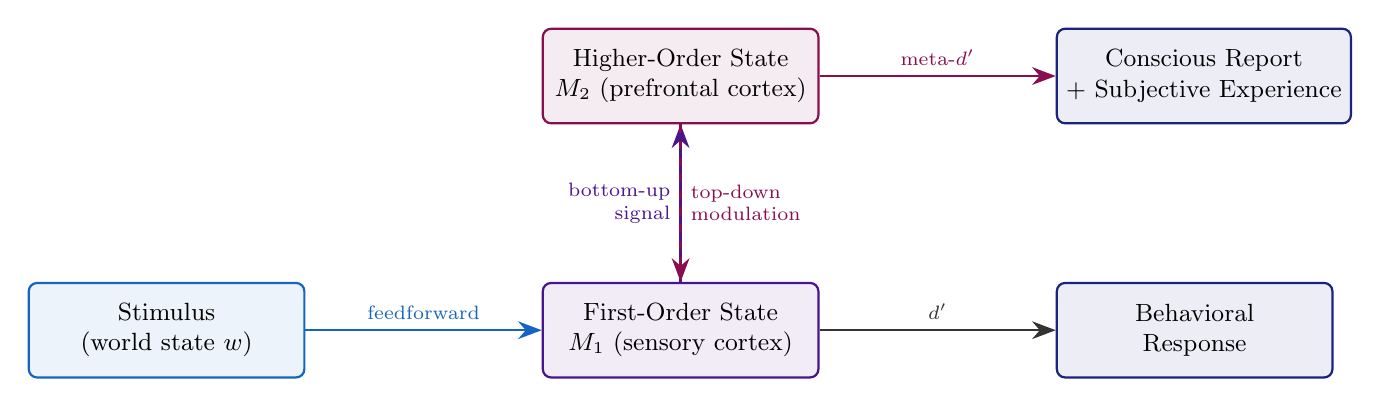
\begin{tikzpicture}[
    box/.style={rectangle, draw=#1, fill=#1!8, thick, minimum width=3.5cm, minimum height=1.2cm, font=\small, align=center, rounded corners=3pt},
    arr/.style={-{Stealth[length=3mm]}, thick},
    node distance=2cm,
  ]
  % Nodes
  \node[box=defcolor] (stim) {Stimulus\\(world state $w$)};
  \node[box=mechcolor, right=3cm of stim] (fo) {First-Order State\\$M_1$ (sensory cortex)};
  \node[box=principlecolor, above=2cm of fo] (ho) {Higher-Order State\\$M_2$ (prefrontal cortex)};
  \node[box=darkindigo, right=3cm of fo] (resp) {Behavioral\\Response};
  \node[box=darkindigo, right=3cm of ho] (report) {Conscious Report\\+ Subjective Experience};

  % Arrows
  \draw[arr, defcolor] (stim) -- node[above, font=\scriptsize] {feedforward} (fo);
  \draw[arr, mechcolor] (fo) -- node[left, font=\scriptsize, align=right] {bottom-up\\signal} (ho);
  \draw[arr, principlecolor, dashed] (ho) -- node[right, font=\scriptsize, align=left] {top-down\\modulation} (fo);
  \draw[arr, darkgray] (fo) -- node[above, font=\scriptsize] {$d'$} (resp);
  \draw[arr, principlecolor] (ho) -- node[above, font=\scriptsize] {meta-$d'$} (report);
\end{tikzpicture}
\end{center}
\vspace{-2pt}
{\small\centering\textit{Figure: Two-level HOT architecture. First-order states in sensory cortex drive behavior; higher-order states in PFC generate conscious experience and report.}\par}

\section{Laminar and Connectivity Considerations}

Recent work has linked higher-order representations to specific \textbf{cortical layers} and \textbf{connection types}:

\begin{itemize}[leftmargin=1.5em]
  \item \textbf{Bottom-up (feedforward):} Layer 2/3 $\to$ layer 4, carried by gamma oscillations. Transmits first-order information to PFC.
  \item \textbf{Top-down (feedback):} Deep layers (5/6) of PFC $\to$ superficial layers (1, 2/3) of sensory cortex, carried by alpha/beta oscillations. Implements the higher-order modulation of first-order states.
  \item \textbf{Prefrontal recurrence:} Within PFC, recurrent excitatory loops (NMDA-dependent) sustain the HOT over time, enabling working memory and deliberate introspection.
\end{itemize}

This architecture is consistent with GNWT's global workspace but adds a specific claim: the PFC activity is not merely broadcasting first-order information but generating a \emph{new representation} (the HOT) with its own content that determines the character of consciousness.


% ══════════════════════════════════════════════════════════════
\chapter{The Computational Framework: SDT and PRM}
% ══════════════════════════════════════════════════════════════

\section{Lau's Signal Detection Model}

Hakwan Lau (2008, 2011) formalized HOT using a two-stage signal detection model that has become the standard computational framework.

\subsection{The Two-Stage Model}

\begin{principlebox}[Lau's Two-Stage SDT Model]
\textbf{Stage 1 (First-Order):} A sensory signal $x_1$ is generated by the stimulus:
\[
  x_1 = \mu_s + \varepsilon_1, \qquad \varepsilon_1 \sim \mathcal{N}(0, \sigma_1^2)
\]
where $\mu_s = d'_1$ for signal-present and $\mu_s = 0$ for signal-absent trials. The first-order sensitivity is $d'_1 = \mu_s / \sigma_1$.

\textbf{Stage 2 (Higher-Order):} A metacognitive readout $x_2$ is generated from $x_1$:
\[
  x_2 = x_1 + \varepsilon_2, \qquad \varepsilon_2 \sim \mathcal{N}(0, \sigma_2^2)
\]
The higher-order sensitivity is:
\[
  d'_2 = \frac{d'_1}{\sqrt{1 + (\sigma_2/\sigma_1)^2}}
\]
Conscious perception is determined by the higher-order readout $x_2$, not by $x_1$ directly.
\end{principlebox}

The key insight: the second stage adds noise ($\sigma_2^2$), so $d'_2 \leq d'_1$. The higher-order representation is a \emph{degraded} version of the first-order signal. This explains why metacognitive accuracy is typically less than first-order accuracy ($M_{\text{ratio}} < 1$).

\subsection{Criterion Setting and Consciousness}

Consciousness in this model depends on whether $x_2$ exceeds a higher-order criterion $c_2$:

\begin{mathbox}
\vspace{-6pt}
\begin{align}
  \text{Conscious ``seeing'':}\quad & x_2 > c_2 \label{eq:conscious}\\
  \text{Not conscious:}\quad & x_2 \leq c_2 \label{eq:not_conscious}
\end{align}
\vspace{-8pt}
\end{mathbox}

This yields four possible outcomes:

\begin{center}
\renewcommand{\arraystretch}{1.4}
\begin{tabular}{>{\raggedright}p{2.5cm} >{\centering}p{4cm} >{\centering\arraybackslash}p{4cm}}
  \toprule
  & \textbf{Signal Present} & \textbf{Signal Absent} \\
  \midrule
  $x_2 > c_2$ (conscious) & \textcolor{defcolor}{\textbf{Veridical seeing}} & \textcolor{principlecolor}{\textbf{Hallucination}} (false alarm) \\
  $x_2 \leq c_2$ (unconscious) & \textcolor{predcolor}{\textbf{Blindsight}} (miss) & Correct rejection \\
  \bottomrule
\end{tabular}
\end{center}

\textbf{Blindsight:} The first-order signal is present ($x_1$ is strong, the stimulus is processed) but the higher-order readout fails to exceed criterion ($x_2 \leq c_2$). The subject denies seeing but performs above chance when forced to guess---exactly the pattern observed in blindsight patients.

\textbf{Hallucination:} The higher-order system generates a ``yes'' response even without a first-order signal (due to noise $\varepsilon_2$). This corresponds to Rosenthal's ``targetless HOTs.''

\subsection{Relating to meta-$d'$}

The meta-$d'$ framework (Maniscalco \& Lau, 2012) provides a way to estimate the higher-order sensitivity:

\begin{mathbox}
\vspace{-6pt}
meta-$d'$ is defined as the value of $d'$ that would produce the observed Type 2 (confidence-accuracy) ROC curve if the metacognitive system were an ideal observer with Type 1 sensitivity = meta-$d'$.

If meta-$d' < d'$: the higher-order system loses information (noise in the metacognitive channel).
If meta-$d' = d'$: perfect metacognition (ideal SDT observer).
If meta-$d' > d'$: the higher-order system has access to additional information.
\vspace{-4pt}
\end{mathbox}

The meta-$d'$ framework is computed by fitting Type 2 hit rates and false alarm rates (hits = high confidence on correct trials, false alarms = high confidence on incorrect trials) to an extended SDT model.

\section{The Bayesian Extension: PRM}

Lau (2019) and Fleming (2020) extended the SDT model into a full Bayesian framework:

\subsection{Perceptual Reality Monitoring}

The higher-order system performs Bayesian inference to determine whether the first-order signal corresponds to reality:

\begin{mathbox}
\vspace{-6pt}
\[
  P(\text{stimulus present} \mid x_1, \text{context}) = \frac{P(x_1 \mid \text{present})\, P(\text{present} \mid \text{context})}{\sum_h P(x_1 \mid h)\, P(h \mid \text{context})}
\]
\vspace{-8pt}
\end{mathbox}

The ``context'' includes prior expectations, attentional state, and task demands. The conscious percept is this posterior probability, or more precisely, the Bayesian decision based on it.

\subsection{Hierarchical Bayesian Model}

Fleming (2020) proposed a hierarchical model:

\begin{mathbox}
\vspace{-6pt}
\textbf{Level 1 (Perceptual):}
\begin{align}
  x &\sim \mathcal{N}(d' \cdot s, \; 1) \quad\text{where } s \in \{0, 1\} \\
  \hat{s} &= \mathbb{1}[x > c_1] \quad\text{(perceptual decision)}
\end{align}
\textbf{Level 2 (Metacognitive):}
\begin{align}
  y &\sim \mathcal{N}(\text{meta-}d' \cdot |\hat{s} - 0.5|, \; 1) \\
  \text{confidence} &= \Phi(y) \quad\text{(mapped to [0, 1])}
\end{align}
\textbf{Level 3 (Hierarchical prior):}
\begin{align}
  \log(\text{meta-}d') &\sim \mathcal{N}(\mu_{\text{meta}}, \; \sigma_{\text{meta}}^2) \\
  c_1 &\sim \mathcal{N}(\mu_c, \; \sigma_c^2)
\end{align}
\vspace{-8pt}
\end{mathbox}

This hierarchical Bayesian model (HMeta-d') estimates metacognitive efficiency while accounting for individual variability. It is fit using Markov Chain Monte Carlo (MCMC) methods and provides the most robust estimate of the higher-order representation's fidelity.

\section{Computational Predictions}

The SDT/Bayesian framework makes specific, testable predictions:

\begin{predbox}[Key Computational Predictions]
\begin{enumerate}[leftmargin=1.5em]
  \item \textbf{Criterion shifts change consciousness without changing perception:} Shifting $c_2$ (the higher-order criterion) changes what is consciously seen without changing first-order sensitivity $d'_1$. This can be achieved by manipulating expectations, attention, or PFC activity.
  \item \textbf{Noise in the metacognitive channel explains blindsight:} High $\sigma_2$ (metacognitive noise) means the higher-order system often fails to detect strong first-order signals, producing blindsight-like dissociations.
  \item \textbf{PFC damage reduces meta-$d'$ but not $d'$:} Damaging the higher-order mechanism should impair metacognition while sparing first-order perception.
  \item \textbf{PFC stimulation can create consciousness without stimulus:} Directly activating the higher-order mechanism (e.g., via TMS or microstimulation) should create conscious experiences even without corresponding sensory input (targetless HOTs).
\end{enumerate}
\end{predbox}


% ══════════════════════════════════════════════════════════════
\chapter{Empirical Evidence}
% ══════════════════════════════════════════════════════════════

\section{Blindsight}

\begin{examplebox}[Blindsight: The Paradigmatic Case]
Patients with damage to primary visual cortex (V1) lose conscious vision in the affected visual field (scotoma) but can still discriminate stimuli when forced to guess---performing well above chance on orientation, motion, and even emotional expression tasks.

\textbf{HOT interpretation:} The first-order visual signal bypasses V1 via subcortical routes (superior colliculus $\to$ pulvinar $\to$ extrastriate cortex), preserving first-order processing ($d' > 0$). However, the higher-order representation in PFC is disrupted (because it normally receives input via V1-mediated pathways), so the patient has no conscious experience ($x_2 \leq c_2$).

This is perhaps the strongest evidence for a two-level architecture: the first-order system works, but without the higher-order representation, there is no consciousness.
\end{examplebox}

\section{Metacognition-Perception Dissociations}

\subsection{Lau \& Passingham (2006)}

Using metacontrast masking with equated $d'$:
\begin{itemize}[leftmargin=1.5em]
  \item Two conditions: same first-order performance ($d'$ equated) but different subjective visibility.
  \item Higher subjective visibility $\to$ greater dlPFC activity.
  \item Same sensory cortex activity across conditions.
  \item Conclusion: PFC generates a higher-order representation that determines subjective experience, independent of first-order processing.
\end{itemize}

\subsection{Rounis et al.\ (2010)}

TMS to dlPFC:
\begin{itemize}[leftmargin=1.5em]
  \item Reduced subjective visibility (shift in $c_2$) without affecting $d'$.
  \item Demonstrates a \emph{causal} role of PFC in the higher-order component.
\end{itemize}

\subsection{Fleming et al.\ (2010, 2014)}

\begin{itemize}[leftmargin=1.5em]
  \item Individual differences in metacognitive accuracy (meta-$d'/d'$) correlate with aPFC gray matter volume and white matter integrity.
  \item aPFC lesions impair metacognitive accuracy while leaving perceptual $d'$ intact.
\end{itemize}

\section{Confidence and Consciousness}

HOT predicts a tight link between \textbf{confidence} (a graded higher-order assessment) and \textbf{consciousness} (a categorical higher-order state). Evidence:

\begin{itemize}[leftmargin=1.5em]
  \item Stimuli rated as ``not seen'' but correctly discriminated (blindsight-like performance in normal subjects) are associated with low confidence.
  \item The transition from ``not seen'' to ``seen'' is associated with a sharp increase in confidence, consistent with a criterion-based mechanism.
  \item Manipulations that increase confidence (e.g., post-cues, reward) can increase reports of ``seeing'' even when $d'$ is unchanged.
\end{itemize}

\section{Neural Oscillatory Evidence}

\begin{mechbox}[Prefrontal Beta/Gamma and Consciousness]
Studies by Gaillard et al.\ (2009) and Panagiotaropoulos et al.\ (2012) show:
\begin{itemize}[leftmargin=1.5em]
  \item Conscious perception is associated with late ($>$200 ms) \textbf{prefrontal gamma} activity, not early sensory gamma.
  \item Prefrontal gamma is sustained for the duration of conscious experience.
  \item Prefrontal beta-band activity ($\sim$15--30 Hz) during the pre-stimulus period predicts whether a stimulus will be consciously perceived, consistent with a top-down metacognitive bias.
\end{itemize}
\end{mechbox}

\section{The No-Report Paradigm Challenge}

A major challenge to HOT (and GWT) comes from ``no-report'' paradigms:

\begin{objbox}[The No-Report Challenge]
When report-related confounds are removed (e.g., by not requiring subjects to report and instead inferring consciousness from neural markers), prefrontal activity associated with consciousness is \textbf{greatly reduced} (Frässle et al., 2014; Pitts et al., 2014).

This suggests that PFC activity may reflect \emph{post-perceptual} processing (report preparation, monitoring) rather than consciousness itself---undermining the core prediction of both HOT and GWT.
\end{objbox}

\textbf{HOT response:} Lau and colleagues argue that no-report paradigms don't eliminate the HOR---they merely eliminate the \emph{report}. The subject still has a higher-order representation (and is still conscious); it's just that the additional processing required for report is removed. The reduced PFC signal may reflect the reporting component, but the metacognitive component (which is more subtle) may still be present but harder to detect.


% ══════════════════════════════════════════════════════════════
\chapter{HOT vs.\ Other Theories}
% ══════════════════════════════════════════════════════════════

\section{HOT vs.\ Global Workspace Theory}

\begin{compbox}[Key Differences: HOT vs.\ GWT]
\renewcommand{\arraystretch}{1.4}
\begin{tabular}{>{\raggedright}p{3cm} >{\raggedright}p{5cm} >{\raggedright\arraybackslash}p{5cm}}
  \toprule
  \textbf{Dimension} & \textbf{HOT / PRM} & \textbf{GWT / GNWT} \\
  \midrule
  What makes a state conscious? & Having a HOR about it & Being broadcast globally \\
  Role of PFC & Generates the HOR (metacognitive) & Part of the workspace (broadcast) \\
  Misrepresentation & Possible (HOR can err) & Not emphasized \\
  Blindsight & Missing HOR, intact first-order & Missing broadcast \\
  Key measure & meta-$d'$ & PCI / P3b amplitude \\
  Consciousness type & Depends on HOR accuracy & All-or-none ignition \\
  Possible overlap & HOR \emph{is} the broadcast? & Broadcast generates HOR? \\
  \bottomrule
\end{tabular}
\end{compbox}

HOT and GWT share the prediction that prefrontal cortex is essential for consciousness. They may converge: perhaps the ``global broadcast'' in GWT \emph{is} the mechanism by which the HOR is generated, or the HOR is what the broadcast \emph{produces}. However, they differ on the possibility of misrepresentation and on the emphasis placed on metacognition.

\section{HOT vs.\ Integrated Information Theory}

\begin{compbox}[Key Differences: HOT vs.\ IIT]
\renewcommand{\arraystretch}{1.4}
\begin{tabular}{>{\raggedright}p{3cm} >{\raggedright}p{5cm} >{\raggedright\arraybackslash}p{5cm}}
  \toprule
  \textbf{Dimension} & \textbf{HOT / PRM} & \textbf{IIT} \\
  \midrule
  Starting point & Cognitive / philosophical & Phenomenological axioms \\
  Key brain area & Prefrontal cortex & Posterior cortex \\
  Misrepresentation & Central feature & Not possible ($\Phi$ = experience) \\
  Panpsychism & No & Yes \\
  Hard Problem & Addressed via explaining function & Claimed identity \\
  Unconscious states & Exist (no HOR) & $\Phi = 0$ \\
  Key conflict & PFC necessity vs.\ sufficiency of posterior cortex \\
  \bottomrule
\end{tabular}
\end{compbox}

The sharpest disagreement is over the role of prefrontal cortex: HOT says PFC is essential; IIT says the posterior cortex ``hot zone'' suffices. This is a testable difference central to the adversarial collaboration.

\section{HOT vs.\ Recurrent Processing Theory}

\begin{compbox}[Key Differences: HOT vs.\ RPT]
\renewcommand{\arraystretch}{1.4}
\begin{tabular}{>{\raggedright}p{3cm} >{\raggedright}p{5cm} >{\raggedright\arraybackslash}p{5cm}}
  \toprule
  \textbf{Dimension} & \textbf{HOT / PRM} & \textbf{RPT (Lamme)} \\
  \midrule
  Minimal NCC & PFC + sensory cortex & Sensory cortex alone \\
  Phenomenal overflow? & No (consciousness $=$ HOR) & Yes (Stage 2 without report) \\
  Report $=$ consciousness? & Close to yes & No \\
  Local recurrence & Unconscious & Phenomenally conscious \\
  Metacognition role & Essential (is consciousness) & Optional (for access only) \\
  \bottomrule
\end{tabular}
\end{compbox}

RPT claims local recurrent processing in sensory cortex creates phenomenal consciousness without any higher-order representation. HOT denies this: without a HOR, recurrent processing is merely unconscious information processing. The debate centers on whether ``consciousness without report'' is coherent.


% ══════════════════════════════════════════════════════════════
\chapter{Objections and Responses}
% ══════════════════════════════════════════════════════════════

\section{The Regress Problem}

\begin{objbox}[Objection: Infinite Regress]
If a mental state $M_1$ is conscious only because of a HOR $M_2$, then what makes $M_2$ conscious? If it requires $M_3$, and $M_3$ requires $M_4$, etc., we have an infinite regress.
\end{objbox}

\textbf{Response:} Rosenthal explicitly states that the HOT ($M_2$) need \emph{not be conscious}. An unconscious HOT suffices to make $M_1$ conscious. The regress only arises if we demand that the HOT itself must be conscious, but this demand is precisely what HOT rejects. $M_2$ becomes conscious only if there is a third-order thought $M_3$ about it---but this is \emph{introspection}, not basic consciousness, and it's optional.

\section{The Misrepresentation Problem}

\begin{objbox}[Objection: Radical Misrepresentation]
If the HOT can misrepresent or even occur without a target, then consciousness can be completely disconnected from reality. This seems absurd: how can I have a vivid experience of red when nothing in my visual system is representing red?
\end{objbox}

\textbf{Response:} Rosenthal embraces this consequence. He argues that cases of radical misrepresentation are rare (the HOT mechanism is usually reliable) but possible in principle. Analogously, perception can be illusory (you see a bent stick in water even though the stick is straight)---the HOT can similarly be misleading. Hallucinations, confabulations, and phantom limb pain may be real examples of misrepresenting or targetless HOTs.

\section{The Animal Consciousness Problem}

\begin{objbox}[Objection: Do Animals Have HOTs?]
If consciousness requires \emph{thoughts} about one's own mental states, then organisms without sophisticated conceptual abilities (infants, non-human animals) cannot be conscious. This seems implausible---surely a dog in pain is conscious.
\end{objbox}

\textbf{Responses:}
\begin{enumerate}[leftmargin=2em]
  \item Rosenthal: The HOT need not be linguistically structured or highly conceptual. A simple, implicit ``sense'' that one is in a certain state may suffice. Animals may have simple HOTs.
  \item Carruthers: The dispositional version avoids this problem---animals can be disposed to have HOTs even if they don't actually form them.
  \item Lau/PRM: The higher-order mechanism is a reality-monitoring signal, which even relatively simple nervous systems can implement. Metacognition has been demonstrated in non-human primates and even rats.
\end{enumerate}

\section{The Explanatory Gap}

\begin{objbox}[Objection: HOTs Don't Explain Qualia]
Even if we accept that HOTs make states conscious, this doesn't explain \emph{why} having a HOT about seeing red produces the subjective experience of redness. The Hard Problem remains.
\end{objbox}

\textbf{Response:} Rosenthal argues that the quality-space theory addresses this: the qualitative character of experience is determined by the HOR's content, which places the experience in a quality space. ``Redness'' is a position in the quality space, defined relationally. However, critics argue this merely redescribes the problem without solving it.

\section{The Prefrontal Cortex Debate}

\begin{objbox}[Objection: PFC May Not Be Necessary]
The no-report paradigm, lesion evidence, and the adversarial collaboration suggest that PFC activity may be a post-perceptual correlate of \emph{reporting} rather than a correlate of consciousness itself. Patients with extensive PFC damage can still appear conscious.
\end{objbox}

\textbf{Response:} HOT proponents argue that (a) complete bilateral PFC destruction is extremely rare, so strong conclusions cannot be drawn; (b) subcortical or preserved cortical areas may compensate; (c) no-report paradigms don't eliminate the HOR, only the report; (d) the relevant PFC involvement may be more subtle than what current neuroimaging can detect.

\section{The Zombie Problem}

\begin{objbox}[Objection: Could There Be a ``HOT Zombie''?]
A system could, in principle, have all the relevant higher-order representations without any subjective experience---it processes meta-representations but there is ``nothing it is like'' to be that system. HOTs explain the \emph{function} of consciousness but not the \emph{phenomenology}.
\end{objbox}

\textbf{Response:} This is a version of the Hard Problem that afflicts all functional/mechanistic theories, not just HOTs. Rosenthal argues that once the functional role is properly characterized, the zombie scenario becomes incoherent---to have the right kind of HOT just \emph{is} to be conscious.


% ══════════════════════════════════════════════════════════════
\chapter{Open Questions and Future Directions}
% ══════════════════════════════════════════════════════════════

\section{Empirical Questions}

\begin{enumerate}[leftmargin=2em]
  \item \textbf{Is PFC necessary?} High-resolution causal manipulations (optogenetics, targeted lesions in animal models) could test whether specific PFC subregions are necessary for consciousness.
  \item \textbf{Can meta-$d'$ be modulated independently of $d'$?} Pharmacological or stimulation studies targeting the metacognitive channel specifically.
  \item \textbf{Does metacognition predict subjective experience trial-by-trial?} Single-trial decoding of metacognitive signals from PFC should predict visibility ratings.
  \item \textbf{The role of the pulvinar and thalamus:} These subcortical structures may mediate the link between first-order and higher-order representations.
\end{enumerate}

\section{Theoretical Questions}

\begin{enumerate}[leftmargin=2em]
  \item \textbf{What counts as a ``suitable'' HOR?} The theory needs sharper criteria for what kind of higher-order state suffices for consciousness.
  \item \textbf{How does HOT handle the richness of experience?} If the higher-order system is capacity-limited, how does it represent the richness of perceptual experience?
  \item \textbf{Can HOT be integrated with other theories?} HOT and GWT may be complementary (the workspace generates HOTs). HOT and predictive processing may converge (the higher-order signal is a prediction about one's own state).
  \item \textbf{Artificial consciousness:} If a machine has a suitable higher-order monitoring system, would it be conscious according to HOT? This has implications for AI ethics.
\end{enumerate}

\section{The Adversarial Collaboration}

The ongoing adversarial collaboration (Melloni et al., 2021) is designed to test predictions that distinguish HOT/GWT (which both predict PFC involvement) from IIT/RPT (which predict posterior cortex sufficiency). Preliminary results suggest that:
\begin{itemize}[leftmargin=1.5em]
  \item Early posterior activity ($\sim$100--250 ms) correlates with consciousness (consistent with IIT/RPT).
  \item Late prefrontal activity ($>$300 ms) is present but reduced in no-report conditions (ambiguous for HOT/GWT).
  \item The results so far do not definitively settle the debate but are generating important constraints on all theories.
\end{itemize}


% ══════════════════════════════════════════════════════════════
\chapter{Further Reading and References}
% ══════════════════════════════════════════════════════════════

\section*{Core HOT Publications}
\begin{enumerate}[label={[\arabic*]}, leftmargin=2.5em]
  \item Rosenthal, D.\ M.\ (1986). Two concepts of consciousness. \textit{Philosophical Studies}, 49(3), 329--359.
  \item Rosenthal, D.\ M.\ (2005). \textit{Consciousness and Mind}. Oxford University Press.
  \item Rosenthal, D.\ M.\ (2012). Higher-order awareness, misrepresentation, and function. \textit{Philosophical Transactions of the Royal Society B}, 367(1594), 1424--1438.
  \item Lau, H.\ \& Rosenthal, D.\ (2011). Empirical support for higher-order theories of conscious awareness. \textit{Trends in Cognitive Sciences}, 15(8), 365--373.
  \item Brown, R., Lau, H., \& LeDoux, J.\ E.\ (2019). Understanding the higher-order approach to consciousness. \textit{Trends in Cognitive Sciences}, 23(9), 754--768.
\end{enumerate}

\section*{Computational and Neural Models}
\begin{enumerate}[label={[\arabic*]}, leftmargin=2.5em, start=6]
  \item Lau, H.\ (2008). A higher order Bayesian decision theory of consciousness. \textit{Progress in Brain Research}, 168, 35--48.
  \item Lau, H.\ \& Passingham, R.\ E.\ (2006). Relative blindsight in normal observers and the neural correlate of visual consciousness. \textit{PNAS}, 103(49), 18763--18768.
  \item Fleming, S.\ M.\ \& Daw, N.\ D.\ (2017). Self-evaluation of decision-making: a general Bayesian framework for metacognitive computation. \textit{Psychological Review}, 124(1), 91--114.
  \item Fleming, S.\ M.\ (2020). Awareness as inference in a higher-order state space. \textit{Neuroscience of Consciousness}, 2020(1), niz020.
  \item Maniscalco, B.\ \& Lau, H.\ (2012). A signal detection theoretic approach for estimating metacognitive sensitivity from confidence ratings. \textit{Consciousness and Cognition}, 21(1), 422--430.
\end{enumerate}

\section*{Metacognition and Prefrontal Cortex}
\begin{enumerate}[label={[\arabic*]}, leftmargin=2.5em, start=11]
  \item Fleming, S.\ M., Weil, R.\ S., Nagy, Z., Dolan, R.\ J., \& Rees, G.\ (2010). Relating introspective accuracy to individual differences in brain structure. \textit{Science}, 329(5998), 1541--1543.
  \item Fleming, S.\ M., et al.\ (2014). Metacognition: computation, biology and function. \textit{Philosophical Transactions of the Royal Society B}, 367(1594).
  \item Rounis, E., Maniscalco, B., Rothwell, J.\ C., Passingham, R.\ E., \& Lau, H.\ (2010). Theta-burst transcranial magnetic stimulation to the prefrontal cortex impairs metacognitive visual awareness. \textit{Cognitive Neuroscience}, 1(3), 165--175.
  \item Miyamoto, K., et al.\ (2017). Causal neural network of metamemory for retrospection in primates. \textit{Science}, 355(6321), 188--193.
\end{enumerate}

\section*{Variants and Philosophical Discussions}
\begin{enumerate}[label={[\arabic*]}, leftmargin=2.5em, start=15]
  \item Lycan, W.\ G.\ (1996). \textit{Consciousness and Experience}. MIT Press.
  \item Kriegel, U.\ (2009). \textit{Subjective Consciousness: A Self-Representational Theory}. Oxford University Press.
  \item Carruthers, P.\ (2000). \textit{Phenomenal Consciousness: A Naturalistic Theory}. Cambridge University Press.
  \item Block, N.\ (1995). On a confusion about a function of consciousness. \textit{Behavioral and Brain Sciences}, 18(2), 227--247.
  \item Van Gulick, R.\ (2004). Higher-order global states (HOGS): an alternative higher-order model. In \textit{Higher-Order Theories of Consciousness}, R.\ J.\ Gennaro (Ed.), 67--92.
\end{enumerate}

\section*{Experimental Evidence and Challenges}
\begin{enumerate}[label={[\arabic*]}, leftmargin=2.5em, start=20]
  \item Weiskrantz, L.\ (1986). \textit{Blindsight: A Case Study and Implications}. Oxford University Press.
  \item Gaillard, R., et al.\ (2009). Converging intracranial markers of conscious access. \textit{PLoS Biology}, 7(3), e1000061.
  \item Frässle, S., Sommer, J., Jansen, A., Naber, M., \& Einhäuser, W.\ (2014). Binocular rivalry: frontal activity relates to introspection and action but not to perception. \textit{Journal of Neuroscience}, 34(5), 1738--1747.
  \item Pitts, M.\ A., Metzler, S., \& Hillyard, S.\ A.\ (2014). Isolating neural correlates of conscious perception from neural correlates of reporting one's perception. \textit{Frontiers in Psychology}, 5, 1078.
  \item Melloni, L., et al.\ (2021). Making the hard problem of consciousness easier. \textit{Science}, 372(6545), 911--912.
\end{enumerate}

\section*{General Reviews}
\begin{enumerate}[label={[\arabic*]}, leftmargin=2.5em, start=25]
  \item Seth, A.\ K.\ \& Bayne, T.\ (2022). Theories of consciousness. \textit{Nature Reviews Neuroscience}, 23, 439--452.
  \item Gennaro, R.\ J.\ (Ed.) (2004). \textit{Higher-Order Theories of Consciousness: An Anthology}. John Benjamins.
  \item LeDoux, J.\ E.\ \& Brown, R.\ (2017). A higher-order theory of emotional consciousness. \textit{PNAS}, 114(10), E2016--E2025.
  \item Dehaene, S., Lau, H., \& Kouider, S.\ (2017). What is consciousness, and could machines have it? \textit{Science}, 358(6362), 486--492.
\end{enumerate}

\vfill
\begin{center}
  {\color{gray}\rule{0.4\textwidth}{0.5pt}}\\[8pt]
  {\small\color{gray}\itshape End of Document}
\end{center}

\end{document}
